\section{Theorie}
Das Rastertunnelmikroskop (RTM) ist ein Gerät welches verwendet wird die Topografien von Oberflächen abzubilden. Das Grundprinzip basiert auf dem Quantenmechanischen Tunneleffekt welcher durch das heranfahren einer Nadel an die Oberfläche so wie dem anlegen eines Potentials zwischen den beiden auftritt.
\subsection{Quantenmechanischer Tunneleffekt}
Der Tunneleffekt beschreibt den Effekt das Teilchen durch Potentialbarrieren durch können auch wenn sie es klassisch nicht könnten.
\begin{figure}[ht]
	% unnumbered tikz *-*:
	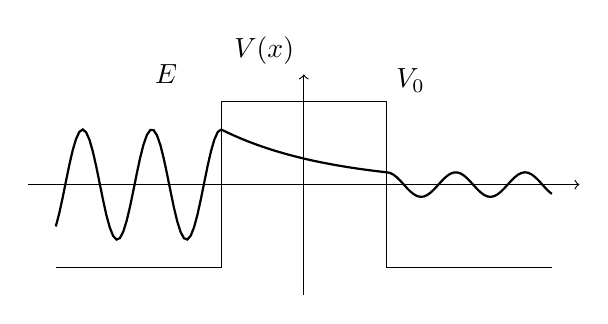
\begin{tikzpicture}[scale=.7]
	\draw (-4.5,-1.5) -| (-1.5,1.5) -- (1.5,1.5) |- (4.5,-1.5);
	\draw[domain=-4.5:-1.5, samples=50, thick] plot (\x, {cos(((\x + 1.5) * 5) r)});
	\draw[domain=-1.5:1.5, samples=50, thick] plot (\x, {exp(-(\x + 1.5) * 0.5)});
	% 0,135335283
	% 0,22313016
	\draw[domain=1.5:4.5, samples=50, thick] plot (\x, {0.22313016 * cos(((\x - 1.5) * 5) r)});
	\draw[->] (-5,0) -- (5,0);
	\draw[->] (0,-2) -- (0,2) node[anchor=south east] {$ V(x) $};
	\node (E) at (-2.5,2) {$ E $};
	\node[anchor=south west] (v) at (1.5,1.5) {$ V_0 $};
	\end{tikzpicture}
	\centering
	\caption{Tunneleffekt bei einer Potentialbarriere $V(x)$\cite{Ex3Tex}}
	\label{Tunneleffekt}
\end{figure}
Innerhalb der Barriere nimmt die Aufenthaltswahrscheinlichkeit des Teilchens exponentiell ab. Die Transmissionswahrscheinlichkeit der Teilchen, die aus der Schrödingergleichung resultiert, ist
abhängig von der Energie des Teilchens und der Breite der Barriere.\par
\subsection{Tunneleffekt am RTM}
Bei leitenden Metallen gibt es eine hohe Anzahl an freien Elektronen. Wenn ein Potential zischen Oberfläche und Nadel angelegt wird fließt ein Strom. Dieser wird Tunnelstrom genannt und entsteht durch dass Tunneln von Elektronen aus besetzten Zuständen von der Probe zur Spitze. Bildlich wird der Effekt in Abbildung \ref{TunnelM} dargestellt.
\begin{figure}[ht]
	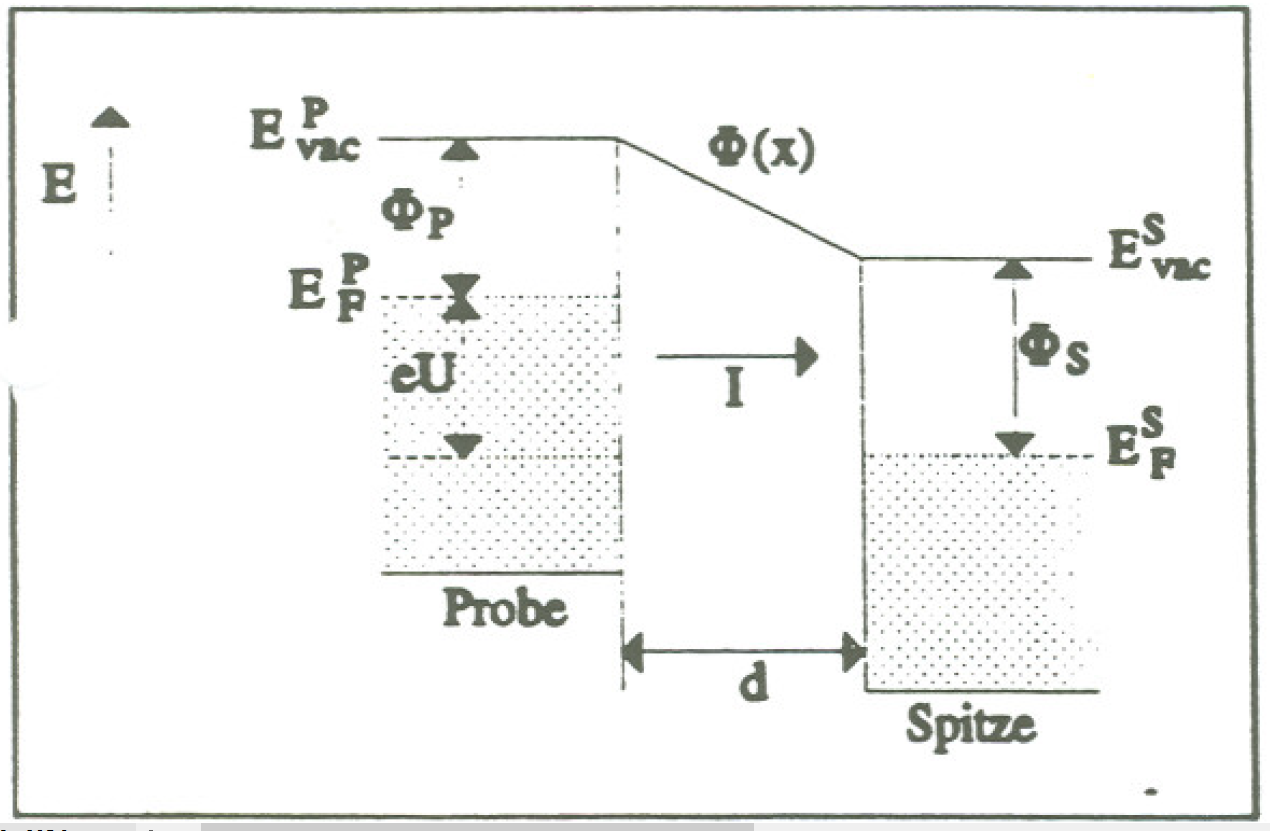
\includegraphics[scale=0.4]{Bild/TunnelstromM}
	\centering
	\caption[Tunneleffekt zwischen Leiter und Spitze bei Metallen]{Tunneleffekt zwischen Leiter und Spitze bei Metallen. $E_F$ ist hierbei die Fermienergie, $\phi$ die Austrittsarbeit.\cite{Staatsexam}}
	\label{TunnelM}
\end{figure}
Der Strom hängt wie in Gleichung \ref{G_M} dargestellt exponentiell vom Abstand d der Probe zur Spitze ab. Die Gleichung gilt bei kleinen Spannungen $eU\ll\phi,\quad eU\ll E_F$.\par
\begin{equation}
	I\propto U\cdot e^{-\sqrt{\frac{2\pi\phi}{\hbar}d}}
	\label{G_M}
\end{equation}
Da bei Halbleitern das Ferminiveau in der Energielücke und nicht im Leitungsband liegt, wird eine
größere extern angelegte Spannung benötigt um einen Tunnelstrom hervorzurufen. Bei hohen Spannungen sind jedoch die Energieabhängigkeiten komplexer. Die Abbildungen \ref{TunnelHL} und \ref{TunnelHL2} zeigen das Bändermodel für den Fall des Tunnelübergangs zwischen Halbleiter und Metall für unterschiedliche Polaritäten der angelegten Spannung.\\
\ \\
\begin{minipage}[t]{0.5\textwidth}
	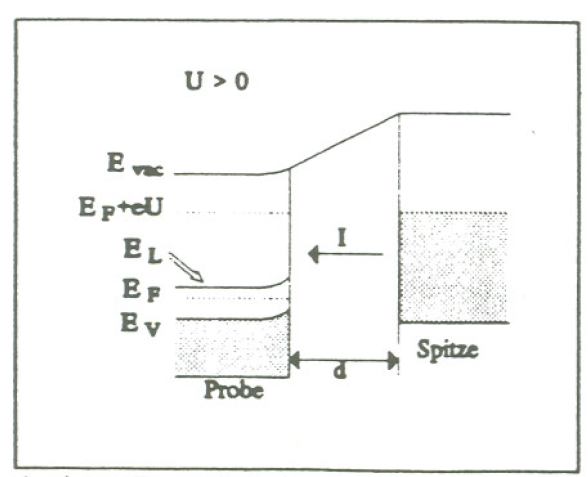
\includegraphics[scale=0.75]{Bild/TunnelspannungML}
	\captionsetup{width=0.8\textwidth}
	\captionof{figure}{Tunneleffekt zischen Halbleiter und Metall bei positiver Spannung gegenüber der Spitze.\cite{Staatsexam}}
	\label{TunnelHL}
\end{minipage}
\begin{minipage}[t]{0.5\textwidth}
	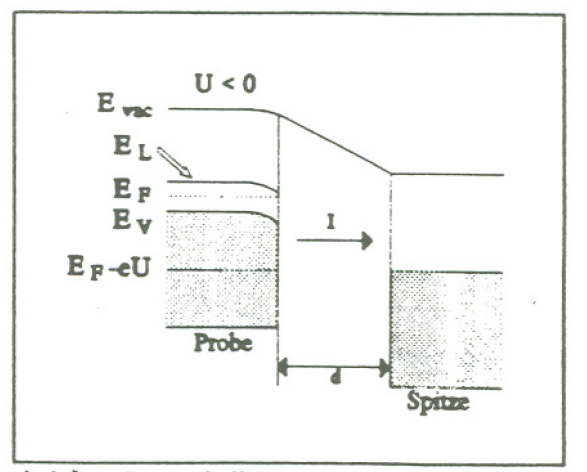
\includegraphics[scale=0.75]{Bild/TunnelspannungML2}
	\captionsetup{width=0.8\textwidth}
	\captionof{figure}{Tunneleffekt zischen Halbleiter und Metall bei negativer Spannung gegenüber der Spitze.\cite{Staatsexam}}
	\label{TunnelHL2}
\end{minipage}\\
\ \\
\ \\
Deshalb kann die gerade verwendete Näherung nicht verwendet werden. 
In einer Erweiterung des Tersoff-Hamann-Modells lässt sich der Tunnelstrom
$I_T$ angeben als:
\begin{equation}
	I_T\propto\int_{E_F}^{E_F+eU}\rho(\vec{r_0},E)dE
\end{equation}
\subsection{Piezokristalle}
Piezokristalle sind Kristalle, die durch anlegen einer Spannung ihre Form verändern. Dieser Effekt beruht darauf, dass sich die im Kristall enthaltenen elektrischen Dipole im elektrischen Feld ausrichten und dadurch für eine Längenvergrößerung des Kristalls in einer Richtung und zeitgleich für eine Längenkontraktion des Kristalls in einer anderen Richtung sorgen. Umgekehrt lässt sich mit
Piezokristallen durch mechanisches Verformen auch eine Spannung erzeugen.
Mit ihnen lässt sich eine präzise Bewegung der Nadel erzeugen. 
\subsection{Rückkopplung}
Das RTM ist mit einem Rückkopplungssystem in Form eines elektronischen Regelkreises
ausgestattet. Eine Erhöhung des Tunnelstroms führt zu einer Erhöhung des Abstands von der Probe. Umgekehrt wird der Abstand zwischen Spitze und Probe bei Abnahme des Tunnelstroms verringert. Die Rückkopplung ermöglicht die Topographie der Oberfläche nachzufahren.
\subsection{Arbeitsmodi des RTM}
Ein RTM hat Grundsätzlich zwei Arbeitsmodi 'Constant Current Mode' und 'Constant Hight Mode'.
\subsubsection{Constant Current Mode}
Beim Constant Current Mode wird der Tunnelstrom konstant gehalten und die Höhe verändert. Beim vermessen der Oberfläche wird eine Spannung $U_z$ verwendet welche ein Maß für die absolute Höhe der Spitze über der Probe ist. Die Methode ist genauer aber da die Nadel vorsichtig beim überqueren der Oberfläche seien muss ist die Methode recht langsam. 
\subsubsection{Constant Hight Mode}
Beim Constant Hight Mode wird die der Abstand zur Oberfläche konstant gehalten. Die Topografie wird daher durch die Veränderung des Tunnelstroms vermessen. Die Methode ist nur nützlich wenn die Oberfläche relativ glatt ist da in dieser Methode die Spitze nicht in der Lage ist auszuweichen. Der Vorteil ist dass sie schneller ist als der Constant Current Mode.
\subsection{Graphit}
Graphit gehört den Halbmetallen an. Es besteht aus Schichten von sechseckig
miteinander verknüpften $sp^2$ hybridisierten Kohlenstoffatomen. In der obersten Schicht gibt es zwei Gruppen von Kohlenstoffatomen, die im Folgenden als $\alpha$-
und $\beta$-Atome bezeichnet werden. Die $\alpha$-Atome der obersten Schicht liegen direkt
über einem Atom der zweiten Schicht. Die $\beta$-Atome der obersten Schicht
hingegen liegen über  'Löchern' der zweiten Schicht. Abbildung \ref{Graphit} zeigt die Struktur von Graphit. Die Kopplung der $\beta$-Atome
bewirkt eine Absenkung der Energie der Energie dieser Atome. Da nur Elektronen
nahe der Fermienergie am Tunnelprozess teilhaben, kann man erwarten,
dass das RTM eine dreieckige Struktur aus $\beta$-Atomen, statt einer sechseckigen
Struktur darstellt.
\begin{figure}[ht]
	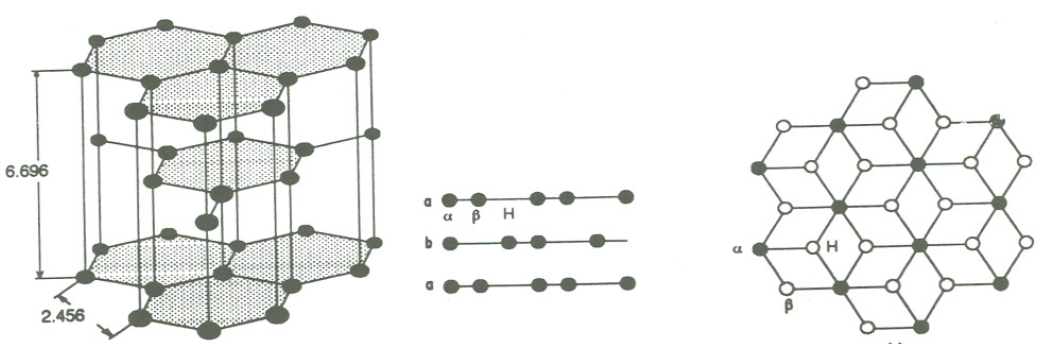
\includegraphics[scale=0.9]{Bild/Graphit}
	\centering
	\caption[Graphit]{Aufbau von Graphit so wie Aufteilung in $\alpha$ und $\beta$-Atome}
	\label{Graphit}
\end{figure}
\subsection{Gold}
Gold als ein Metall hat eine Leitfähigkeit welche durch frei bewegliche Elektronen entsteht. Diese machen jedoch die Messung schwer da sich eine Art Elektronengas bildet. Es ist daher leichter die Oberfläche in einem größeren Bereich anzuschauen in Form von Elektronen Wolken zu beobachten. Ein Beispiel ist hier aus der Anleitung\cite{anleitung} in Abbildung \ref{GoldBsp} zu sehen.
\begin{figure}[ht]
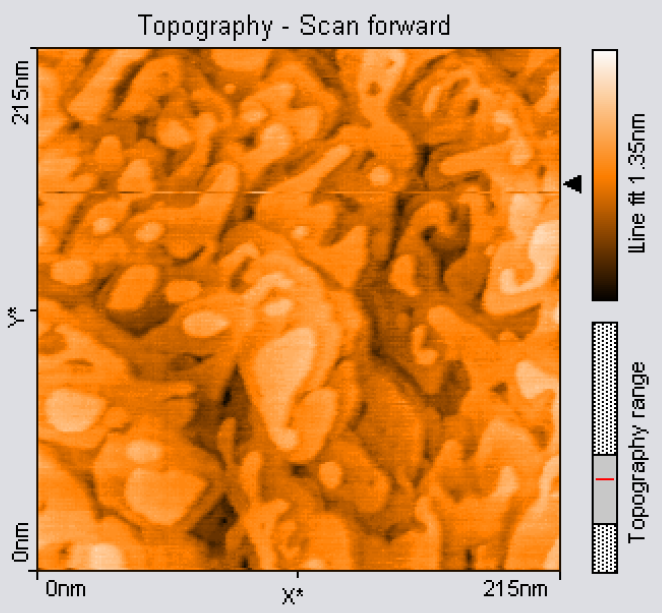
\includegraphics[scale=0.5]{Bild/GoldBsp}
\centering
\caption{Beispiel für die erwartete Elektronenwolken Struktur bei Gold.}
\label{GoldBsp}
\end{figure} 
\subsection{Molybdändisulfid}
Molybdändisulfid ist ein Vertreter der Halbleiter. $MoS_2$ ist schichtartig aufgebaut.
Auf eine Schicht Molybdändisulfid folgen jeweils zwei Schichten Schwefel. Die
Schwefelatome sind in Form eines Gitters mit einer Gitterkonstanten $g = 3.16$\,\AA
angeordnet. Die Molybdändisulfid-Schichten sind dazu seitlich versetzt und werden durch
Van-der-Waalskräfte zusammengehalten.
\section{Versuchsdurchführung}
Für den Versuch wurde als erstes das RTM und ein Computer zum Auslesen der Informationen eingeschaltet. Zur Erstellung der Spitze, welche zur Abtastung verwendet wird, wird PtIr Draht verwendet. Hierfür muss der Draht so abgetrennt werden, dass die Spitze wenige Atome dick ist. Um die Güte der Spitze zu testen wurde die Probe erst einmal an einer Graphit Probe getestet, da diese besonders leicht zu untersuchen ist. Hierfür wird eine Graphit Probe an einem Magneten befestigt welcher dann in das RTM eingesetzt wird. Diese wird dann auf ein paar Millimeter von Hand herangeschoben. Danach wird die Probe mechanisch langsam herangefahren bis man über einen Spiegel keine Lücke zwischen Probe und Spitze erkennen kann. Es ist jedoch Vorsicht geboten da die Spitze nicht die Probe berühren darf, da dies die Spitze zerstören würden. Ab diesem Punkt wurde die Approach Methode des RTM genutzt, welche die Probe den restlichen Weg an die Spitze fährt. Dies geht solange bis das System ein Bild anzeigt. Wenn dies trotz beendeten Approach nicht der Fall ist muss entweder eine neue Spitze erstellt werden oder der Vorgang erneut gestartet werden. Sobald ein Bild erkannt wird kann getestet werden ob die Spitze Sinnvoll ist oder nicht. Hierfür wurden Hinweise aus der Betriebsanleitung des Geräts verwendet\cite{RMT}. Als Modus des RTM wird Constant Current Mode verwendet. Dies erlaubt drei Weitere Einstellung unter z-Einstellung. Diese sind P,I und D-Gain welche die Trajektorie der Spitze verändern und damit das Bild verbessern. Sollten diese auch zu nichts führen muss eine neue Spitze verwendet werden. \par Nach dem Testen einiger Spitzen wurde eine gute gefunden mit der die Oberfläche von Graphit gut Aufgelöst werden konnte. Danach wurde die Probe zurückgefahren und und durch Gold ersetzt. Beim Heranfahren ist jedoch die Spitze gegen die Probe gefahren und eine neue Spitze musste erstellt werden und erneut an Graphit getestet werden. Nach dem dies gelang wurden letztendlich auf Gold vermessen bei dem eine Wolken ähnliche Struktur gesehen wurde. Hier wurden für mehrere z- Einstellungen Messungen gespeichert. Als letztes wurde die Molybdändisulfid Probe vermessen. Hier wurde jedoch schnell klar das die Nadel nicht geeignet war die Oberfläche sinnvoll aufzulösen.
\section{Auswertung}
\subsection{Graphit}
Für Graphit soll der Gitterparameter $a=2.456 \,$nm bestimmt werden welcher in links in Abbildung \ref{Graphit} eingezeichnet ist. Dieser Parameter beschriebt den Abstand zwischen zwei $\alpha$ oder $\beta$ Atomen. Hierfür wurden die in Abbildung \ref{1}, \ref{2} dargestellten Messungen von den beiden funktionierenden Spitzen verwendet.
Hierbei wurde das Programm \verb|Gwyddion| verwendet um die Abstände der Atome zu bestimmen.
Um Fehler zu verringern werden mehrere Atomabstände $a$ auf einmal gemessen. Der Fehler auf den Abstand $x_{Abst}$ wurde auf $\sigma_{x}=0.05\,$nm geschätzt.
\begin{equation}
	a = \frac{x_{Abst}}{n}
\end{equation}
\begin{equation*}
	\sigma_{a} = \frac{\sigma_{x}}{n_{Atome}}
\end{equation*}
Die Einzelnen Werte für $x_{Abst}$ sind in Tabelle \ref{Werte} notiert.
\begin{figure}[ht]
	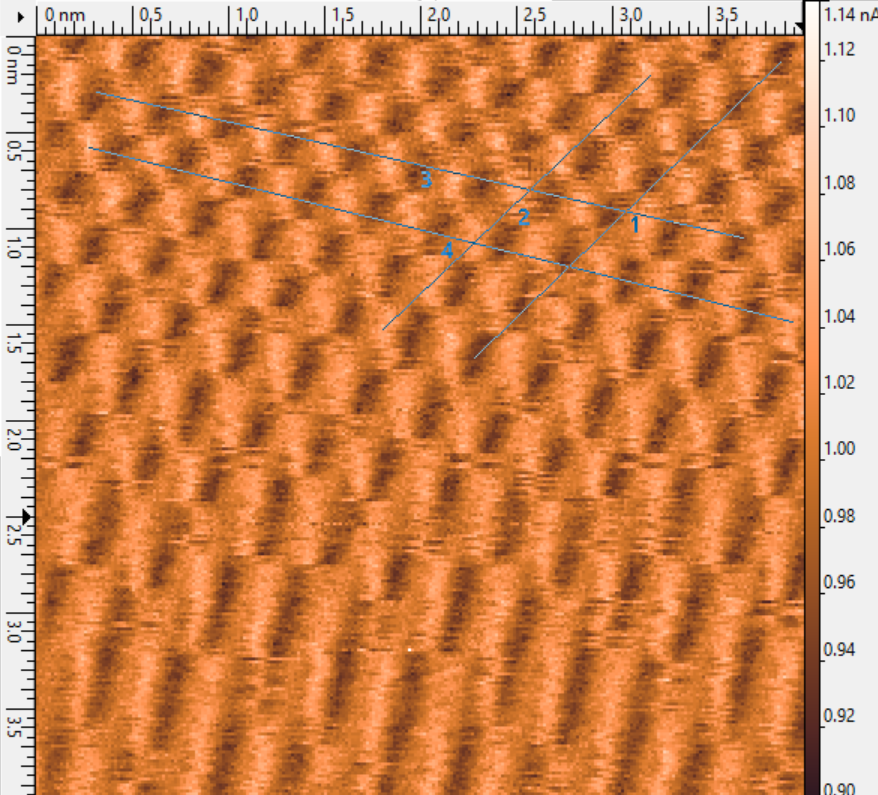
\includegraphics[scale=0.7]{Bild/Graphit2}
	\centering
	\caption[Messung von Graphit bei Spitze 1]{ Graphit Messung der ersten Spitze mit 4 Messreihen bei $4$\,nm. Die Parameter bei dieser Messung waren:  $P=4500$, $I=500$, $D=0$, $\frac{P}{L}=256$ und $\frac{T}{L}=0.2\,$s.}
	\label{1}
\end{figure}
\begin{figure}[ht]
	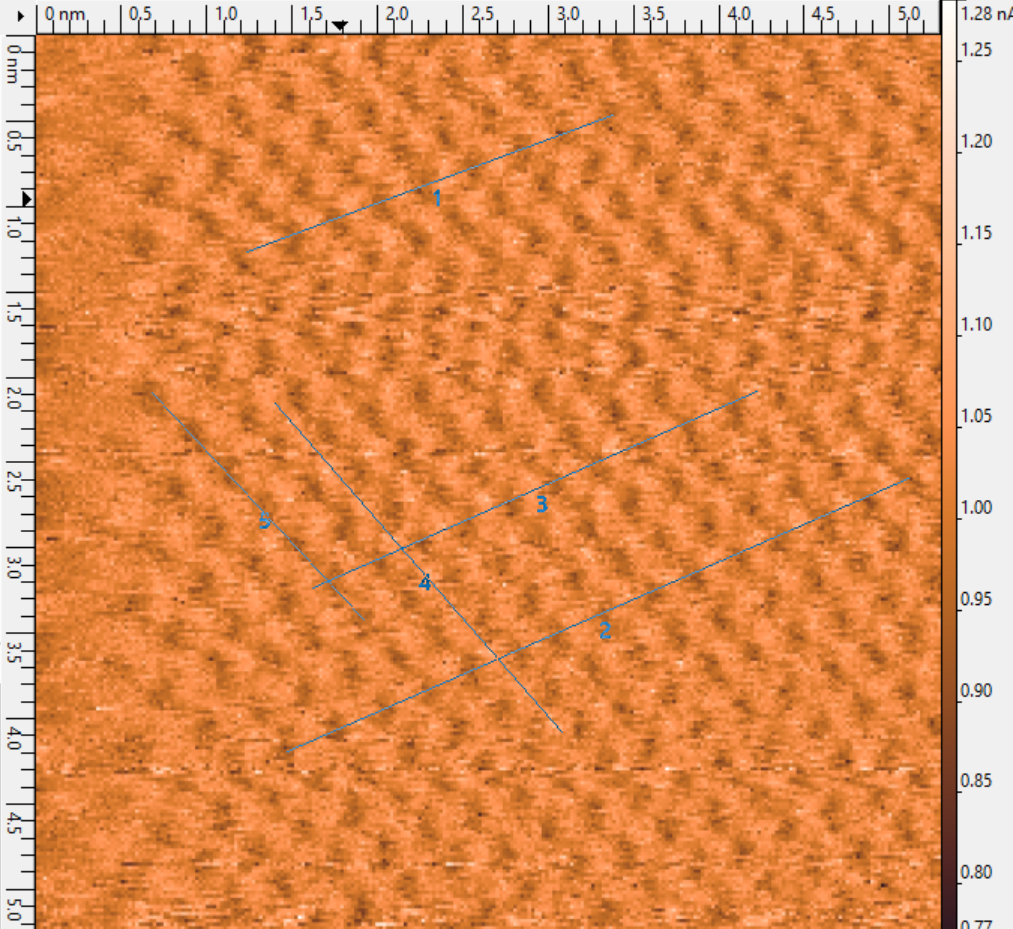
\includegraphics[scale=0.6]{Bild/Graphit4}
	\centering
	\caption[Messung von Graphit bei Spitze 2]{ Graphit Messung der zweiten Spitze mit 5 Messreihen bei $5.3$\,nm. Die Parameter bei dieser Messung waren:  $P=2300$, $I=400$, $D=0$, $\frac{P}{L}=256$ und $\frac{T}{L}=0.1\,$s.}
	\label{2}
\end{figure}
\begin{table}[ht]
	\begin{Dtabular}[1.1]{|c|c|c|c|c|}
		\hline
		Abbildung&Messreihe&Abstand $x_{Abst}$ [nm]& Anzahl an Atome$-1$&Gitterparameter $a$ [nm]\\
		\hline
		Erste Spitze&1&$2.22\pm0.05$&$7$&$0.278 \pm 0.006$\\
		\hline
		Erste Spitze&2&$1.92\pm0.05$&$6$&$0.274 \pm 0.007$\\
		\hline
		Erste Spitze&3&$3.45\pm0.05$&$10$&$0.314 \pm 0.005$\\
		\hline
		Erste Spitze&4&$3.77\pm0.05$&$11$&$0.314 \pm 0.004$\\
		\hline
		Zweite Spitze&1&$2.29\pm0.05$&$8$&$0.254 \pm 0.006$\\
		\hline
		Zweite Spitze&2&$3.97\pm0.05$&$14$&$0.2647 \pm 0.0033$\\
		\hline
		Zweite Spitze&3&$2.84\pm0.05$&$10$&$0.258 \pm 0.005$\\
		\hline
		Zweite Spitze&4&$2.55\pm0.05$&$9$&$0.255 \pm 0.005$\\
		\hline
		Zweite Spitze&5&$1.82\pm0.05$&$6$&$0.260 \pm 0.007$\\
		\hline
	\end{Dtabular}
	\centering
	\caption[Messwerte]{Messung}
	\label{Werte}
\end{table}
\FloatBarrier
Aus den Werten Gitterparametern wird nun der Mittelwert  berechnet und dessen Fehler mit \\Gleichung \ref{Mittelwert}. 
\begin{equation}
	\sigma_{\bar{x}}=\sqrt{\frac{\frac{1}{n-1}\sum_{i=1}^{n}\left(x_i-\bar{x}\right)^2}{n}}
	\label{Mittelwert}
\end{equation}
Hiermit ergeben sich für Abbildung \ref{1} mit Spitze eins und Abbildung \ref{2} von Spitze zwei folgende Werte:
\begin{equation*}
	a_{S1}=(0.295\pm 0.011)\,\text{nm}
\end{equation*}
\begin{equation*}
	a_{S2}=(0.2585\pm0.0019)\,\text{nm}
\end{equation*}
\subsection{Gold}
Beim nutzten der Nadel für Gold konnte nach Einstellen des z-Controller eine Abbildung gefunden werden welche Elektronen Wolken abbildete. Diese ist in Abbildung \ref{Gold} zu finden.
\begin{figure}[ht]
	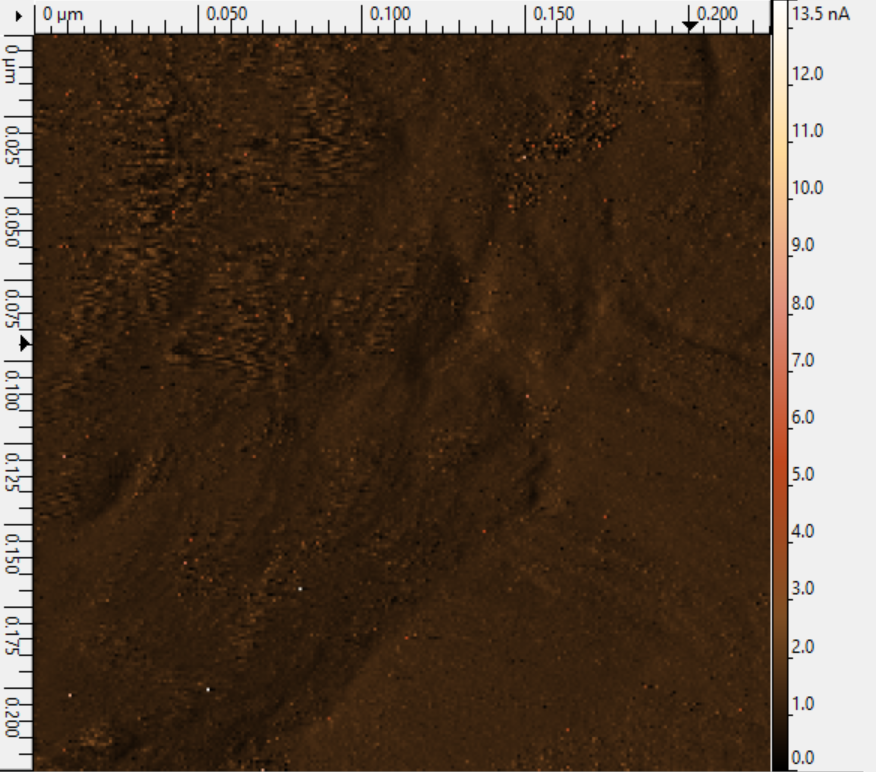
\includegraphics[scale=0.5]{Bild/Gold}
	\centering
	\caption[Messung von Gold]{Messung für die Goldprobe mit möglicher Weise erkennbaren Elektronenwolken. Einstellgrößen waren für diese Messung: $P=2500$, $I=400$, $D=0$, $\frac{P}{L}=256$ und $\frac{T}{L}=0.3\,$s.}
	\label{Gold}
\end{figure}\\
Zusätzlich wurden für Gold mehrere Messungen durchgeführt mit unterschiedlichen Einstellungen von P-Gain D-Gain und I-Gain Einstellungen.
Leider konnte aus den Aufnahmen keine Sinnvollen Schlüsse gezogen werden, da sie sich scheinbar unregelmäßig veränderten. Die Abbildungen sind der Vollständigkeit halber im Anhang zu finden.\par
\newpage
\subsection{Molybdändisulfid}
Auch für Molybdändisulfid wurde die Nadel getestet. Hier wurde jedoch kein gute Auflösung für die Atomare Struktur gefunden. Außerdem ist wie in Abbildung \ref{Mol} und \ref{Mol2} zu erkennen ist die Nadel vermutlich nicht gut genug gewesen. Dies lässt sich an dem eher Streifen artigen Muster erkennen.
\begin{figure}[ht]
	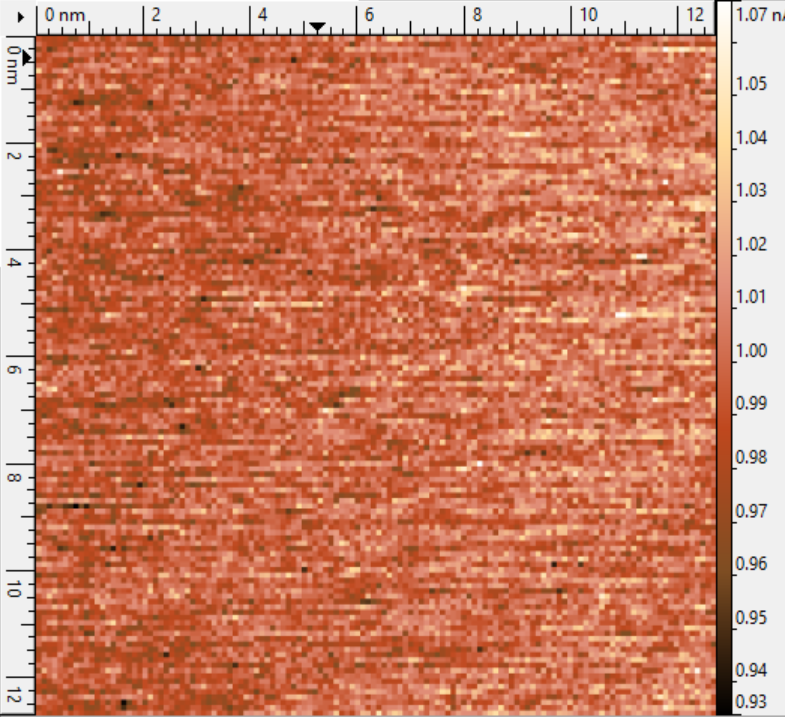
\includegraphics[scale=0.62]{Bild/Mol}
	\centering
	\caption[Messung von Molybdändisulfid 1]{Messung von Molybdändisulfid bei $12.7\,$nm mit $P=3900$, $I=800$, $D=0$, $\frac{P}{L}=128$ und $\frac{T}{L}=0.1\,$s.}
	\label{Mol}
\end{figure}
\begin{figure}[ht]
	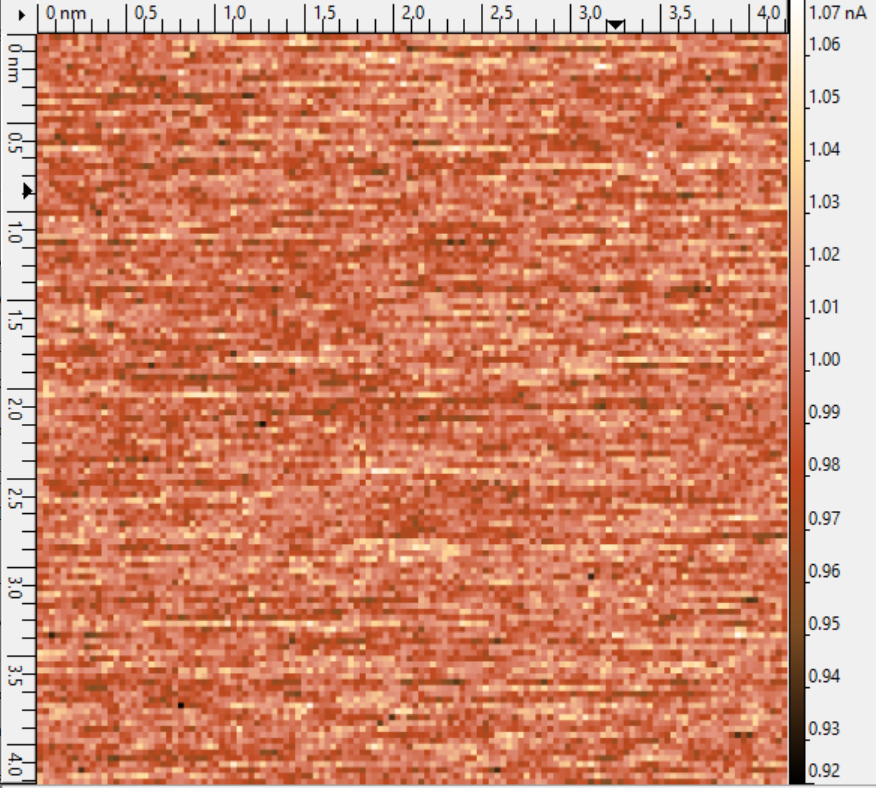
\includegraphics[scale=0.57]{Bild/Mol2}
	\centering
	\caption[Messung von Molybdändisulfid 2]{Messung von Molybdändisulfid bei $4.22\,$nm mit $P=3900$, $I=800$, $D=0$, $\frac{P}{L}=128$ und $\frac{T}{L}=0.1\,$s.}
	\label{Mol2}
\end{figure}
\FloatBarrier
\newpage
\section{Diskussion}
\subsection{Aufgetretene Probleme und Mögliche Fehlergründe}
Als aller erstes ist natürlich die Spitze ein Grund für Ungenauigkeiten und Fehler. Dies liegt daran das der Herstellungsprozess bei der, der Draht auf eine Spitze mit wenigen Atomen gekürzt wird recht unzuverlässig ist und es zu großen Teilen auf Glück basiert ob man eine funktionierende Spitze erhält. \par
Zusätzlich hat das Testen einer Nadel recht viel Zeit gekostet da das heranfahren oftmals mehrere Versuche gekostet hat. Hierbei konnte es zusätzlich leicht passieren dass die Spitze an die Probe geriet und dabei unbrauchbar wurde.\par
Als weitere mögliches Fehlerquelle welches auftreten kann ist die Qualität der Proben. Diese können entweder verunreinigt sein oder durch Fett oder Kratzer unbrauchbar werden. Bei den hier verwendeten Proben war dies jedoch eher eine geringere Fehler Quelle da die Proben besonders die Graphit Probe relativ neu waren.\par
Eine weiterer Grund für schlechte Ergebnisse können die Einstellungen des z-Controllers sein, welche großen Einfluss auf die Auflösung der Messung haben. Auch die Einstellungen für Pixel/Line und Time/Line können erhebliche Auswirkungen haben. \par
Ein Systematischer Fehler welcher besonders bei der ersten funktionierenden Nadel Probleme bereitet hat war der Thermische Drift. Dieser ist besonders in Abbildung \ref{1} gut an dem scheinbaren länger werden der Atome nach untenhin zu erkennen. Hierbei können schon $0.1^\circ C$ zu einer Längenänderung des Probenhalters von mehreren Nanometern führen\cite{RMT}.\par
Letztlich sind noch mechanische oder elektrische Störungen als Fehlerquellen zu vermerken. Der Aufbau z.B reagiert sehr empfindlich auf Stöße wie das stoßen gegen den Tisch des Versuchsaufbaus. Elektrische Störungen könnten Theoretisch durch Teilchen entstehen welche in den Versuchsaufbau gelangen. 
\subsection{Ergebnisse}
Die zwei für Graphit berechneten Gitterparameter sind:
\begin{equation*}
a_{S1}=(0.295\pm 0.011)\,\text{nm}
\end{equation*}
\begin{equation*}
a_{S2}=(0.2585\pm0.0019)\,\text{nm}
\end{equation*}
Der erwartete Literatur Wert liegt bei, $a=0.2456\,$nm. Wenn man diesen mit der Formel \ref{vgl} vergleicht erhält man für $a_{S1}$ $t=4.49$ und für $a_{S2}$ $t=6.79$.
Beide Werte sind unverträglich mit dem Literaturwert. Dies lässt sich für $a_{S1}$ durch den Thermischen Drift erklären welcher hier die Messwerte in y Richtung stark auseinander gezogen hat. Der Grund warum der Mittelwert hier jedoch trotzdem noch besser ist wie der von $a_{S2}$, trotz größerer Differenz, liegt an dem großen Fehler welcher durch die die eben genannten Messreihen verursacht wurde. Aus diesen Gründen sollte der Wert von $a_{S2}=(0.2585\pm0.0019)\,\text{nm}$ trotz schlechterem Vergleichswert der genauere sein.
\begin{equation}
	t=\frac{|x_{Messung}-x_{Literatur}|}{\sigma_{x}}
	\label{vgl}
\end{equation}
Für Gold konnte eine Aufnahme gewonnen werden bei der man die erwarteten Elektronen Wolken erkennen konnte. Jedoch sind sie nicht besonders gut aufgelöst. Dies liegt vermutlich an noch nicht genug optimierten z-Controller Einstellungen und der wahrscheinlich doch nicht ganz so guten Spitze. Diese würde auch das nicht erkennbare Molybdändisulfid so wie einen weiteren möglichen Systematischen Fehler für die Gitterstruktur bei Graphit.